\documentclass[man]{apa6}
\usepackage{lmodern}
\usepackage{amssymb,amsmath}
\usepackage{ifxetex,ifluatex}
\usepackage{fixltx2e} % provides \textsubscript
\ifnum 0\ifxetex 1\fi\ifluatex 1\fi=0 % if pdftex
  \usepackage[T1]{fontenc}
  \usepackage[utf8]{inputenc}
\else % if luatex or xelatex
  \ifxetex
    \usepackage{mathspec}
  \else
    \usepackage{fontspec}
  \fi
  \defaultfontfeatures{Ligatures=TeX,Scale=MatchLowercase}
\fi
% use upquote if available, for straight quotes in verbatim environments
\IfFileExists{upquote.sty}{\usepackage{upquote}}{}
% use microtype if available
\IfFileExists{microtype.sty}{%
\usepackage{microtype}
\UseMicrotypeSet[protrusion]{basicmath} % disable protrusion for tt fonts
}{}
\usepackage{hyperref}
\hypersetup{unicode=true,
            pdftitle={Racial/Ethnic Disparities in Mental Health},
            pdfauthor={Shaina Trevino, Maria Schweer-Collins, Alejandra Garcia Isaza, \& Ernst-August Doelle},
            pdfkeywords={race, ethnicity, mental health disparities, depression, substance use},
            pdfborder={0 0 0},
            breaklinks=true}
\urlstyle{same}  % don't use monospace font for urls
\usepackage{graphicx,grffile}
\makeatletter
\def\maxwidth{\ifdim\Gin@nat@width>\linewidth\linewidth\else\Gin@nat@width\fi}
\def\maxheight{\ifdim\Gin@nat@height>\textheight\textheight\else\Gin@nat@height\fi}
\makeatother
% Scale images if necessary, so that they will not overflow the page
% margins by default, and it is still possible to overwrite the defaults
% using explicit options in \includegraphics[width, height, ...]{}
\setkeys{Gin}{width=\maxwidth,height=\maxheight,keepaspectratio}
\IfFileExists{parskip.sty}{%
\usepackage{parskip}
}{% else
\setlength{\parindent}{0pt}
\setlength{\parskip}{6pt plus 2pt minus 1pt}
}
\setlength{\emergencystretch}{3em}  % prevent overfull lines
\providecommand{\tightlist}{%
  \setlength{\itemsep}{0pt}\setlength{\parskip}{0pt}}
\setcounter{secnumdepth}{0}
% Redefines (sub)paragraphs to behave more like sections
\ifx\paragraph\undefined\else
\let\oldparagraph\paragraph
\renewcommand{\paragraph}[1]{\oldparagraph{#1}\mbox{}}
\fi
\ifx\subparagraph\undefined\else
\let\oldsubparagraph\subparagraph
\renewcommand{\subparagraph}[1]{\oldsubparagraph{#1}\mbox{}}
\fi

%%% Use protect on footnotes to avoid problems with footnotes in titles
\let\rmarkdownfootnote\footnote%
\def\footnote{\protect\rmarkdownfootnote}


  \title{Racial/Ethnic Disparities in Mental Health}
    \author{Shaina Trevino\textsuperscript{1}, Maria
Schweer-Collins\textsuperscript{1}, Alejandra Garcia
Isaza\textsuperscript{1}, \& Ernst-August Doelle\textsuperscript{1}}
    \date{}
  
\shorttitle{Title}
\affiliation{
\vspace{0.5cm}
\textsuperscript{1} University of Oregon}
\keywords{race, ethnicity, mental health disparities, depression, substance use\newline\indent Word count: X}
\usepackage{csquotes}
\usepackage{upgreek}
\captionsetup{font=singlespacing,justification=justified}

\usepackage{longtable}
\usepackage{lscape}
\usepackage{multirow}
\usepackage{tabularx}
\usepackage[flushleft]{threeparttable}
\usepackage{threeparttablex}

\newenvironment{lltable}{\begin{landscape}\begin{center}\begin{ThreePartTable}}{\end{ThreePartTable}\end{center}\end{landscape}}

\makeatletter
\newcommand\LastLTentrywidth{1em}
\newlength\longtablewidth
\setlength{\longtablewidth}{1in}
\newcommand{\getlongtablewidth}{\begingroup \ifcsname LT@\roman{LT@tables}\endcsname \global\longtablewidth=0pt \renewcommand{\LT@entry}[2]{\global\advance\longtablewidth by ##2\relax\gdef\LastLTentrywidth{##2}}\@nameuse{LT@\roman{LT@tables}} \fi \endgroup}


\DeclareDelayedFloatFlavor{ThreePartTable}{table}
\DeclareDelayedFloatFlavor{lltable}{table}
\DeclareDelayedFloatFlavor*{longtable}{table}
\makeatletter
\renewcommand{\efloat@iwrite}[1]{\immediate\expandafter\protected@write\csname efloat@post#1\endcsname{}}
\makeatother
\usepackage{lineno}

\linenumbers

\authornote{

Correspondence concerning this article should be addressed to Shaina
Trevino, Postal address. E-mail:
\href{mailto:my@email.com}{\nolinkurl{my@email.com}}}

\abstract{
Sign Up:

One or two sentences providing a \textbf{basic introduction} to the
field, comprehensible to a scientist in any discipline.

Two to three sentences of \textbf{more detailed background},
comprehensible to scientists in related disciplines.

One sentence clearly stating the \textbf{general problem} being
addressed by this particular study.

One sentence summarizing the main result (with the words ``\textbf{here
we show}'' or their equivalent).

Two or three sentences explaining what the \textbf{main result} reveals
in direct comparison to what was thought to be the case previously, or
how the main result adds to previous knowledge.

One or two sentences to put the results into a more \textbf{general
context}.

Two or three sentences to provide a \textbf{broader perspective},
readily comprehensible to a scientist in any discipline.


}

\begin{document}
\maketitle

\section{Introduction}\label{introduction}

Despite advances in access to health services, quality of care, and
overall gains in life expectancy, racial/ethnic disparities in health in
the United States (U.S.) remains to disproportionally affect the lives
of racial/ethnic minority groups. D. R. Williams and Mohammed (2009)
refer to the finding of Levine et al. (2016) that approximately 100,000
African Americans who would not die if there were no racial disparities
die prematurely every year. Unfortunately, in the mental health arena,
racial/ethnic disparities are no exception.

Even though the burden and impact of physical diseases on different
racial/ethnic subgroups have been far more studied than the impact and
burden of mental health disorders, we know that globally, depression is
the leading cause of disability and loss of productivity, and that its
direst outcome, death via suicide, is on the rise (WHO, 2018 (accessed
December 4, 2018)). It is well-known that mental health services are
costly and thus a high proportion of the American population cannot
afford them.

Given that depression is usually screened and treated first in primary
care settings, access to medical care is the first barrier to treatment
that racial/ethnic minority groups face (D. R. Williams \& Mohammed,
2009). From there, racial/ethnic minority groups experience barriers
such as low detection rate of mental health disorders in comparison to
Whites (Borowsky et al., 2000); language barriers for non-English
speakers (Fiscella, Franks, Doescher, \& Saver, 2002); use of screening
measures not translated or validated for racial/ethnic minority groups;
issues of trust related but not limited to underrepresentation of
racial/ethnic minorities among mental health professionals, and cultural
differences in understanding and treating mental health disorders
(Miranda \& Cooper, 2004). Overall, these and other barriers affect the
access and quality of treatment racial/ethnic minority groups receive in
respect to their mental health.

-----Maria will do drug use onset and health disparities (short 1
paragraph) ---- use of substances as an alternative treatment for
depression that people may recur to----

In the present study, we aim to explore some of the health disparities
among different racial/ethnic groups using a nationally representative
sample, the National Health and Nutrition Examination Survey (NHANES)
2015 -- 2016.

NOTE: The WHO reference is not working well. Is showing the access date.

\section{Methods}\label{methods}

Sign up:

We report how we determined our sample size, all data exclusions (if
any), all manipulations, and all measures in the study.

\subsection{Participants}\label{participants}

Sign up:

\subsection{Measures}\label{measures}

sign up:

To assess depression symptoms, we used the depression module from the
full Patient Health Questionnaire (Kroenke, Spitzer, \& Williams, 2001:
PHQ). The PHQ-9 is a 9-item, self-report screening instrument.
Participants are prompted by the stem \enquote{Over the last 2 weeks,
how often have you been bothered by any of the following problems?}.
Sample questions include \enquote{Feeling down, depressed, or hopeless?}
and \enquote{Thoughts that you would be better off dead or of hurting
yourself in some way}. The module uses a 4-point scale that goes from 0
(not at all) to 3 (nearly every day). \enquote{Refuse to answer} and
\enquote{Don't know} options are also included. A single score is
derived from the depression module by summing the responses for the 9
items. Scores can range from 0 to 27; higher scores reflect more severe
depressive symptoms.

Insurance coverage was assessed with the item \enquote{Are you covered
by health insurance or some other kind of health care plan?} from the
NHANES Health Insurance Questionnaire. Response choices included
\enquote{Yes}. \enquote{No}, \enquote{Refused}, and \enquote{Don't
know}.

Usage of mental health services was assessed with the item
\enquote{During the past 12 months, have you seen or talked to a mental
health professional such as a psychologist, psychiatrist, psychiatric
nurse or clinical social worker about your health?} from the NHANES
Hospital Utilization and Access to Care questionnaire. Response choices
included \enquote{Yes}. \enquote{No}, \enquote{Refused}, and
\enquote{Don't know}.

\subsection{Data analysis}\label{data-analysis}

We used R (Version 3.5.1; R Core Team, 2018) and the R-packages
\emph{bindrcpp} (Version 0.2.2; Müller, 2018), \emph{dplyr} (Version
0.7.8; Wickham, François, Henry, \& Müller, 2018), \emph{forcats}
(Version 0.3.0; Wickham, 2018a), \emph{ggplot2} (Version 3.0.0; Wickham,
2016), \emph{here} (Version 0.1; Müller, 2017), \emph{kableExtra}
(Version 0.9.0; Zhu, n.d.), \emph{papaja} (Version 0.1.0.9842; Aust \&
Barth, 2018), \emph{purrr} (Version 0.2.5; Henry \& Wickham, 2018),
\emph{readr} (Version 1.2.1; Wickham, Hester, \& Francois, 2018),
\emph{rio} (Version 0.5.10; C.-h. Chan, Chan, Leeper, \& Becker, 2018),
\emph{stringr} (Version 1.3.1; Wickham, 2018b), \emph{tibble} (Version
1.4.2; Müller \& Wickham, 2018), \emph{tidyr} (Version 0.8.2; Wickham \&
Henry, 2018), and \emph{tidyverse} (Version 1.2.1; Wickham, 2017) for
all our analyses. sign up:

\section{Results}\label{results}

We should use inline code here

Description of plot 1: Alejandra

\begin{verbatim}
## Warning: Removed 425 rows containing missing values (geom_col).
\end{verbatim}

\begin{figure}
\centering
\includegraphics{Final_Paper_Group_3_files/figure-latex/plot1-1.pdf}
\caption{}
\end{figure}

Shaina will describe her plot of drug use by ethnicities
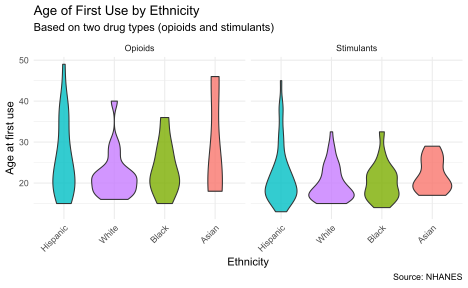
\includegraphics{Final_Paper_Group_3_files/figure-latex/ST_plot1-1.pdf}

plot 2
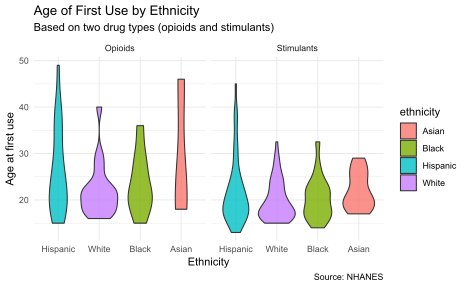
\includegraphics{Final_Paper_Group_3_files/figure-latex/ST_plot-1.pdf}

plot 3
\includegraphics{Final_Paper_Group_3_files/figure-latex/ST_plott-1.pdf}

ST table

\begin{verbatim}
## Warning: Expected 2 pieces. Missing pieces filled with `NA` in 10 rows [1,
## 2, 3, 4, 5, 6, 7, 8, 9, 10].
\end{verbatim}

\begin{table}[tbp]
\begin{center}
\begin{threeparttable}
\caption{\label{tab:ST_table}Average depression score and age of first opioid and stimulant use}
\begin{tabular}{llll}
\toprule
Ethnicity & \multicolumn{1}{c}{Depression Score} & \multicolumn{1}{c}{Opioid Use} & \multicolumn{1}{c}{Stimulant Use}\\
\midrule
Asian & 3.01 & 27.86 & 21.73\\
Black & 3.16 & 22.18 & 20.30\\
Hispanic & 3.29 & 25.81 & 21.43\\
Other/Multiracial & 3.47 & 22.33 & 18.93\\
White & 3.53 & 21.60 & 20.23\\
\bottomrule
\end{tabular}
\end{threeparttable}
\end{center}
\end{table}

\section{Discussion}\label{discussion}

sign up:

Insert one data visualization -- we are using two, I believe Alejandra's
viz. and one from Shaina Exploratory association plot?
\includegraphics{Final_Paper_Group_3_files/figure-latex/ST_plot3-1.pdf}

Insert Table -- JP?

\newpage

\section{References}\label{references}

\begingroup
\setlength{\parindent}{-0.5in} \setlength{\leftskip}{0.5in}

\hypertarget{refs}{}
\hypertarget{ref-R-papaja}{}
Aust, F., \& Barth, M. (2018). \emph{papaja: Create APA manuscripts with
R Markdown}. Retrieved from \url{https://github.com/crsh/papaja}

\hypertarget{ref-borowsky2000risk}{}
Borowsky, S. J., Rubenstein, L. V., Meredith, L. S., Camp, P.,
Jackson-Triche, M., \& Wells, K. B. (2000). Who is at risk of
nondetection of mental health problems in primary care? \emph{Journal of
General Internal Medicine}, \emph{15}(6), 381--388.

\hypertarget{ref-R-rio}{}
Chan, C.-h., Chan, G. C., Leeper, T. J., \& Becker, J. (2018).
\emph{Rio: A swiss-army knife for data file i/o}.

\hypertarget{ref-fiscella2002disparities}{}
Fiscella, K., Franks, P., Doescher, M. P., \& Saver, B. G. (2002).
Disparities in health care by race, ethnicity, and language among the
insured: Findings from a national sample. \emph{Medical Care}, 52--59.

\hypertarget{ref-R-purrr}{}
Henry, L., \& Wickham, H. (2018). \emph{Purrr: Functional programming
tools}. Retrieved from \url{https://CRAN.R-project.org/package=purrr}

\hypertarget{ref-kroenke2001phq}{}
Kroenke, K., Spitzer, R. L., \& Williams, J. B. (2001). The phq-9:
Validity of a brief depression severity measure. \emph{Journal of
General Internal Medicine}, \emph{16}(9), 606--613.

\hypertarget{ref-levine2016black}{}
Levine, R. S., Foster, J. E., Fullilove, R. E., Fullilove, M. T.,
Briggs, N. C., Hull, P. C., \ldots{} Hennekens, C. H. (2016).
Black-white inequalities in mortality and life expectancy, 1933--1999:
Implications for healthy people 2010. \emph{Public Health Reports}.

\hypertarget{ref-miranda2004disparities}{}
Miranda, J., \& Cooper, L. A. (2004). Disparities in care for depression
among primary care patients. \emph{Journal of General Internal
Medicine}, \emph{19}(2), 120--126.

\hypertarget{ref-R-here}{}
Müller, K. (2017). \emph{Here: A simpler way to find your files}.
Retrieved from \url{https://CRAN.R-project.org/package=here}

\hypertarget{ref-R-bindrcpp}{}
Müller, K. (2018). \emph{Bindrcpp: An 'rcpp' interface to active
bindings}. Retrieved from
\url{https://CRAN.R-project.org/package=bindrcpp}

\hypertarget{ref-R-tibble}{}
Müller, K., \& Wickham, H. (2018). \emph{Tibble: Simple data frames}.
Retrieved from \url{https://CRAN.R-project.org/package=tibble}

\hypertarget{ref-R-base}{}
R Core Team. (2018). \emph{R: A language and environment for statistical
computing}. Vienna, Austria: R Foundation for Statistical Computing.
Retrieved from \url{https://www.R-project.org/}

\hypertarget{ref-who}{}
WHO. (2018 (accessed December 4, 2018)). Depression. Retrieved from
\url{http://www.who.int/news-room/fact-sheets/detail/depression}

\hypertarget{ref-R-ggplot2}{}
Wickham, H. (2016). \emph{Ggplot2: Elegant graphics for data analysis}.
Springer-Verlag New York. Retrieved from \url{http://ggplot2.org}

\hypertarget{ref-R-tidyverse}{}
Wickham, H. (2017). \emph{Tidyverse: Easily install and load the
'tidyverse'}. Retrieved from
\url{https://CRAN.R-project.org/package=tidyverse}

\hypertarget{ref-R-forcats}{}
Wickham, H. (2018a). \emph{Forcats: Tools for working with categorical
variables (factors)}. Retrieved from
\url{https://CRAN.R-project.org/package=forcats}

\hypertarget{ref-R-stringr}{}
Wickham, H. (2018b). \emph{Stringr: Simple, consistent wrappers for
common string operations}. Retrieved from
\url{https://CRAN.R-project.org/package=stringr}

\hypertarget{ref-R-tidyr}{}
Wickham, H., \& Henry, L. (2018). \emph{Tidyr: Easily tidy data with
'spread()' and 'gather()' functions}. Retrieved from
\url{https://CRAN.R-project.org/package=tidyr}

\hypertarget{ref-R-dplyr}{}
Wickham, H., François, R., Henry, L., \& Müller, K. (2018). \emph{Dplyr:
A grammar of data manipulation}. Retrieved from
\url{https://CRAN.R-project.org/package=dplyr}

\hypertarget{ref-R-readr}{}
Wickham, H., Hester, J., \& Francois, R. (2018). \emph{Readr: Read
rectangular text data}. Retrieved from
\url{https://CRAN.R-project.org/package=readr}

\hypertarget{ref-williams2009discrimination}{}
Williams, D. R., \& Mohammed, S. A. (2009). Discrimination and racial
disparities in health: Evidence and needed research. \emph{Journal of
Behavioral Medicine}, \emph{32}(1), 20--47.

\hypertarget{ref-R-kableExtra}{}
Zhu, H. (n.d.). \emph{KableExtra: Construct complex table with 'kable'
and pipe syntax}.

\endgroup


\end{document}
